% Created 2018-04-17 Tue 09:08
% Intended LaTeX compiler: pdflatex
\documentclass[10pt]{beamer}
\usepackage[utf8]{inputenc}
\usepackage[T1]{fontenc}
\usepackage{graphicx}
\usepackage{grffile}
\usepackage{longtable}
\usepackage{wrapfig}
\usepackage{rotating}
\usepackage[normalem]{ulem}
\usepackage{amsmath}
\usepackage{textcomp}
\usepackage{amssymb}
\usepackage{capt-of}
\usepackage{hyperref}
\usetheme{Boadilla}
\author{ECON 499: Economic Growth and Development}
\date{Spring 2018}
\title{Population and Growth}
\usecolortheme{seagull}
\usefonttheme[onlylarge]{structurebold}
\usefonttheme[onlymath]{serif}
\setbeamerfont*{frametitle}{size=\normalsize,series=\bfseries}
\setbeamertemplate{navigation symbols}{}
\setbeamertemplate{itemize item}[triangle]
\setbeamertemplate{footline}{}
\setbeamertemplate{enumerate items}[default]
\hypersetup{
 pdfauthor={ECON 499: Economic Growth and Development},
 pdftitle={Population and Growth},
 pdfkeywords={},
 pdfsubject={},
 pdfcreator={Emacs 25.2.2 (Org mode 9.1.6)}, 
 pdflang={English}}
\begin{document}

\maketitle

\begin{frame}[label={sec:org419035e}]{}
\alert{Announcements}
\begin{itemize}
\item Reading
\begin{itemize}
\item Chapters 4
\end{itemize}
\item Meet here on Thursday (no lab)
\item Homework due on Thursday (uploaded to Canvas)
\begin{itemize}
\item Expect technological "hiccups"
\end{itemize}
\end{itemize}
\end{frame}

\begin{frame}[label={sec:orgd88e217}]{}
\alert{Population and growth}
\begin{itemize}
\item More people means more mouths to feed
\item More people also means more workers
\item How does production per capita respond to population growth?
\end{itemize}
\end{frame}

\begin{frame}[label={sec:org3290a85}]{}
\begin{center}
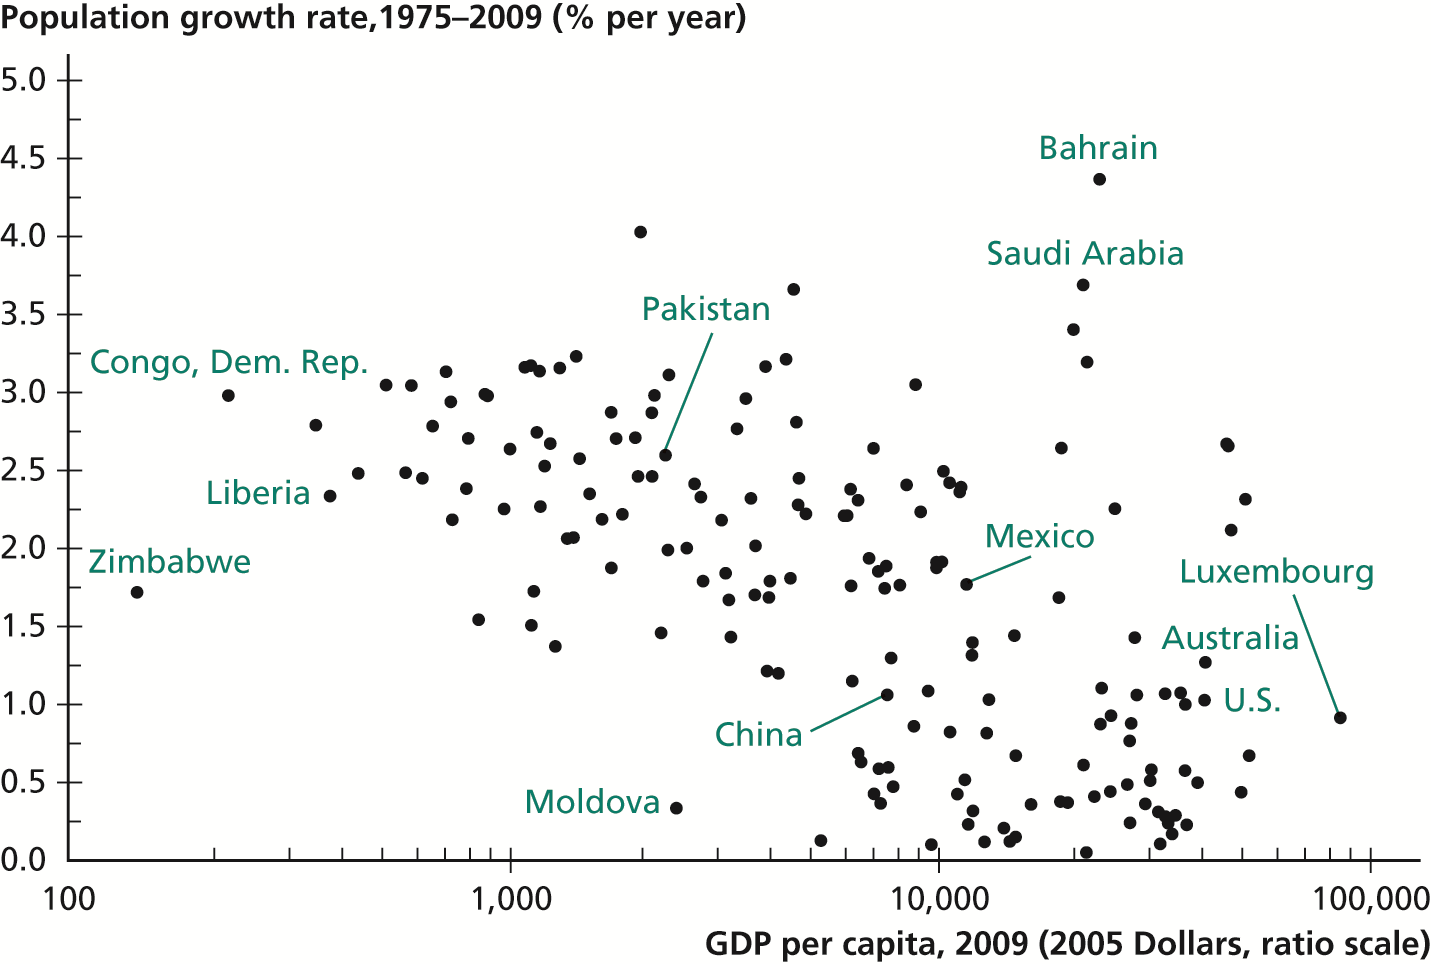
\includegraphics[width=.75\textwidth]{./img/4.1.png}
\end{center}
\end{frame}

\begin{frame}[label={sec:orgfb88509}]{}
\begin{center}
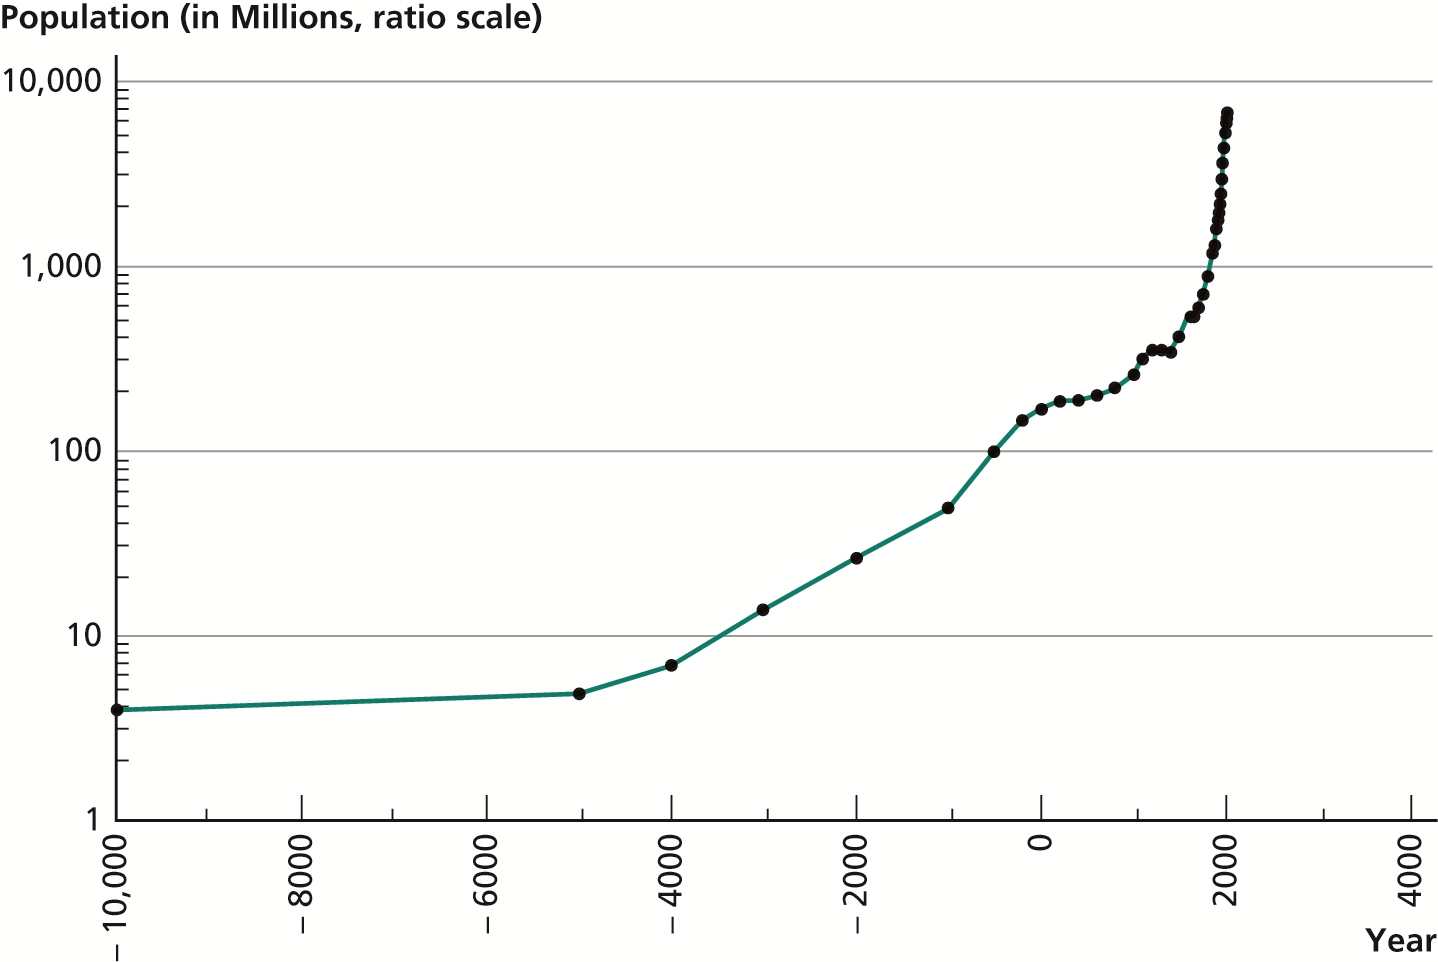
\includegraphics[width=.75\textwidth]{./img/4.2.png}
\end{center}
\end{frame}

\begin{frame}[label={sec:orgf530d5d}]{}
\alert{Malthusian model}
\begin{itemize}
\item Thomas Malthus (1766-1834)
\item Productive resources are \emph{scarce}, sometimes finite (land)
\item As population increases, land per person decreases, making people worse off
\item As poverty increases, people start dying and having fewer children, causing population to fall
\item Population and income are self-regulating, mankind "stuck" at subsistence income level
\item Malthus's solution: "Moral restraint"
\end{itemize}
\end{frame}

\begin{frame}[label={sec:org2b3aa1b}]{Breakdown of the Malthusian Model}
\begin{center}
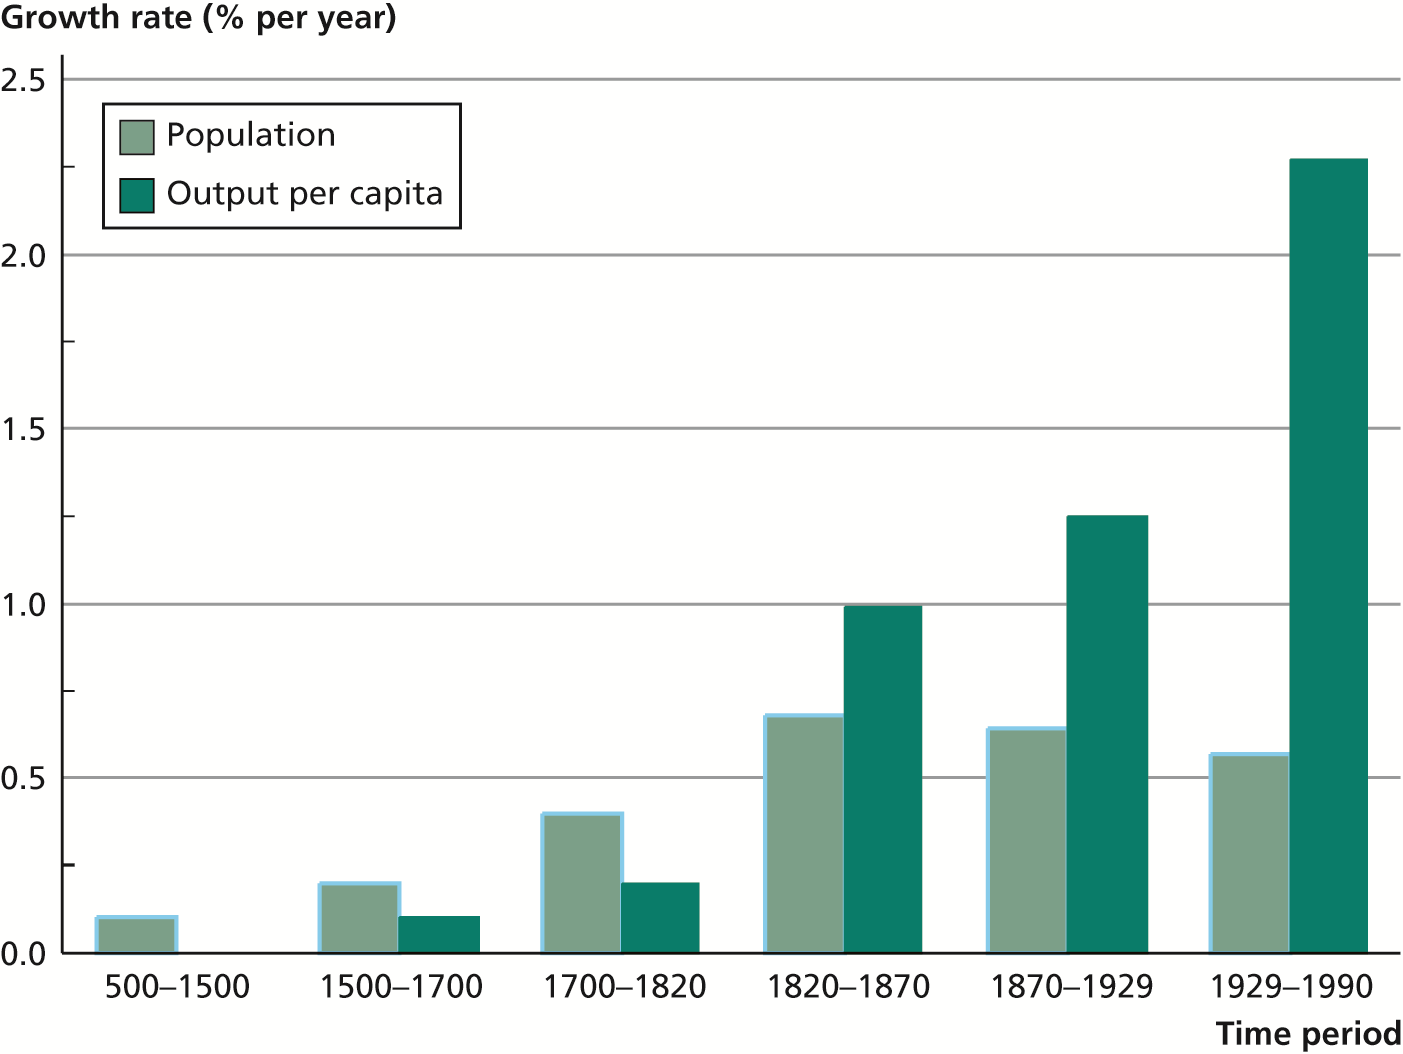
\includegraphics[width=.75\textwidth]{./img/4.6.png}
\end{center}
\end{frame}

\begin{frame}[label={sec:orga0ff42d}]{}
\alert{Explaining population growth}
\begin{itemize}
\item Solow model predicts that increased population growth can decrease income through capital dilution
\item Population growth in Solow model is \emph{exogenous}, determined outside the model
\item Population growth usually modeled as \emph{demographic transition}
\item Developing countries go through mortality and fertility transitions as they develop
\end{itemize}
\end{frame}

\begin{frame}[label={sec:org861daaf}]{}
\alert{Mortality transition}
\begin{itemize}
\item Life expectancy at birth: number of years a newborn baby in a given year will live on average
\item Most countries have seen life expectancy increase over last few centuries, beginning with developed countries
\item Three factors:
\begin{enumerate}
\item More plentiful, nutritious food
\item Public health: sanitation, clean water, etc
\item Medical technology
\end{enumerate}
\end{itemize}
\end{frame}

\begin{frame}[label={sec:org1125624}]{}
\begin{center}
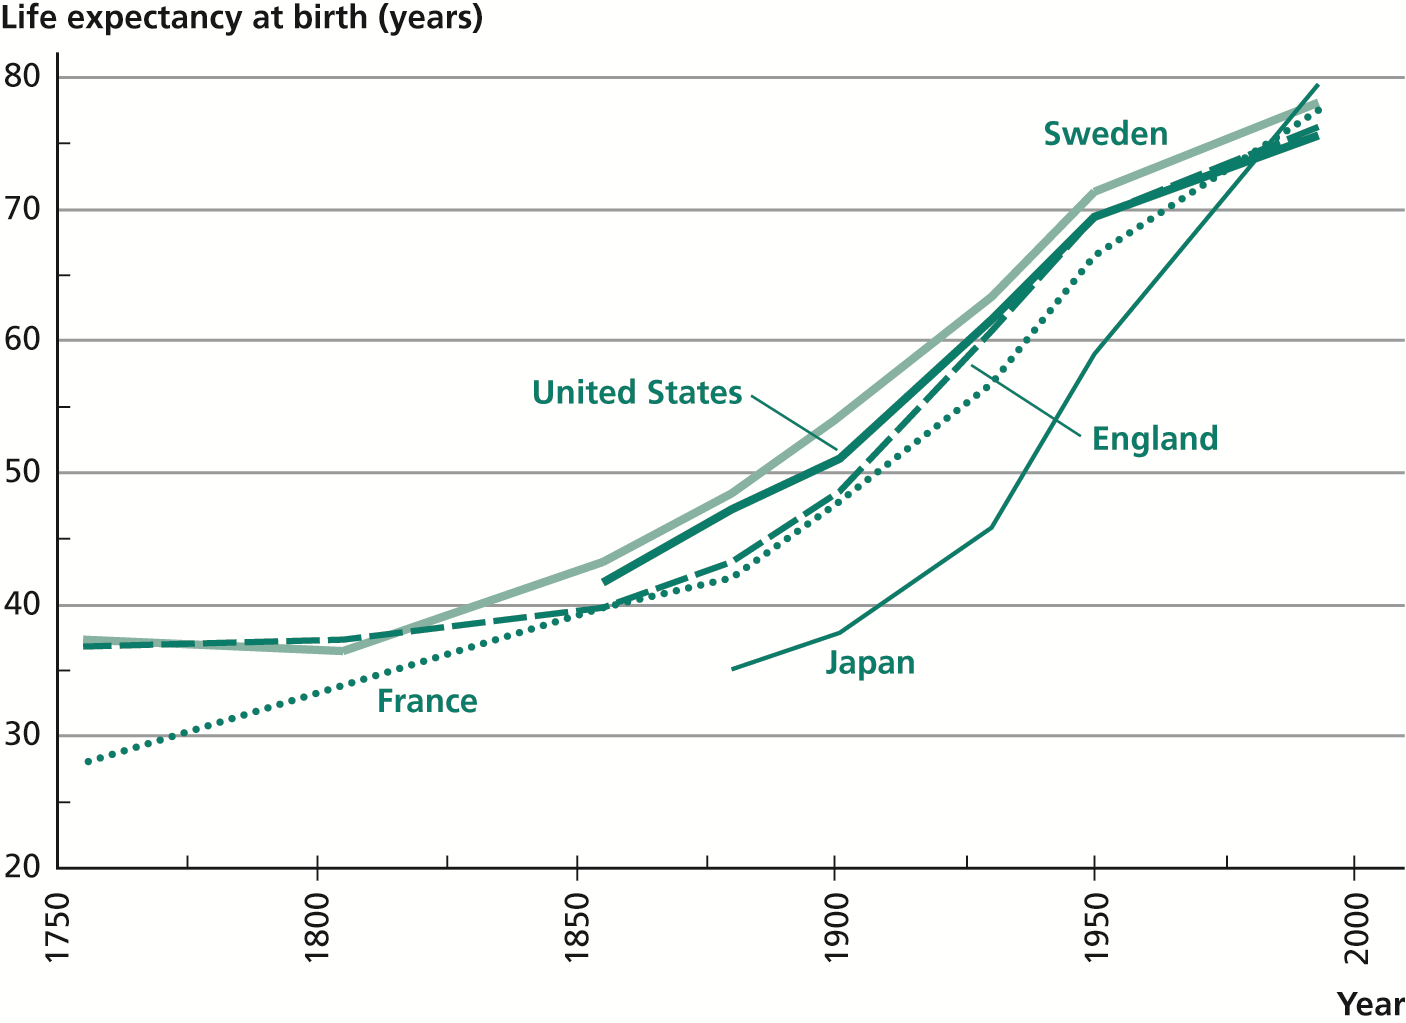
\includegraphics[width=.75\textwidth]{./img/4.8.png}
\end{center}
\end{frame}

\begin{frame}[label={sec:org3446baa}]{}
\begin{center}
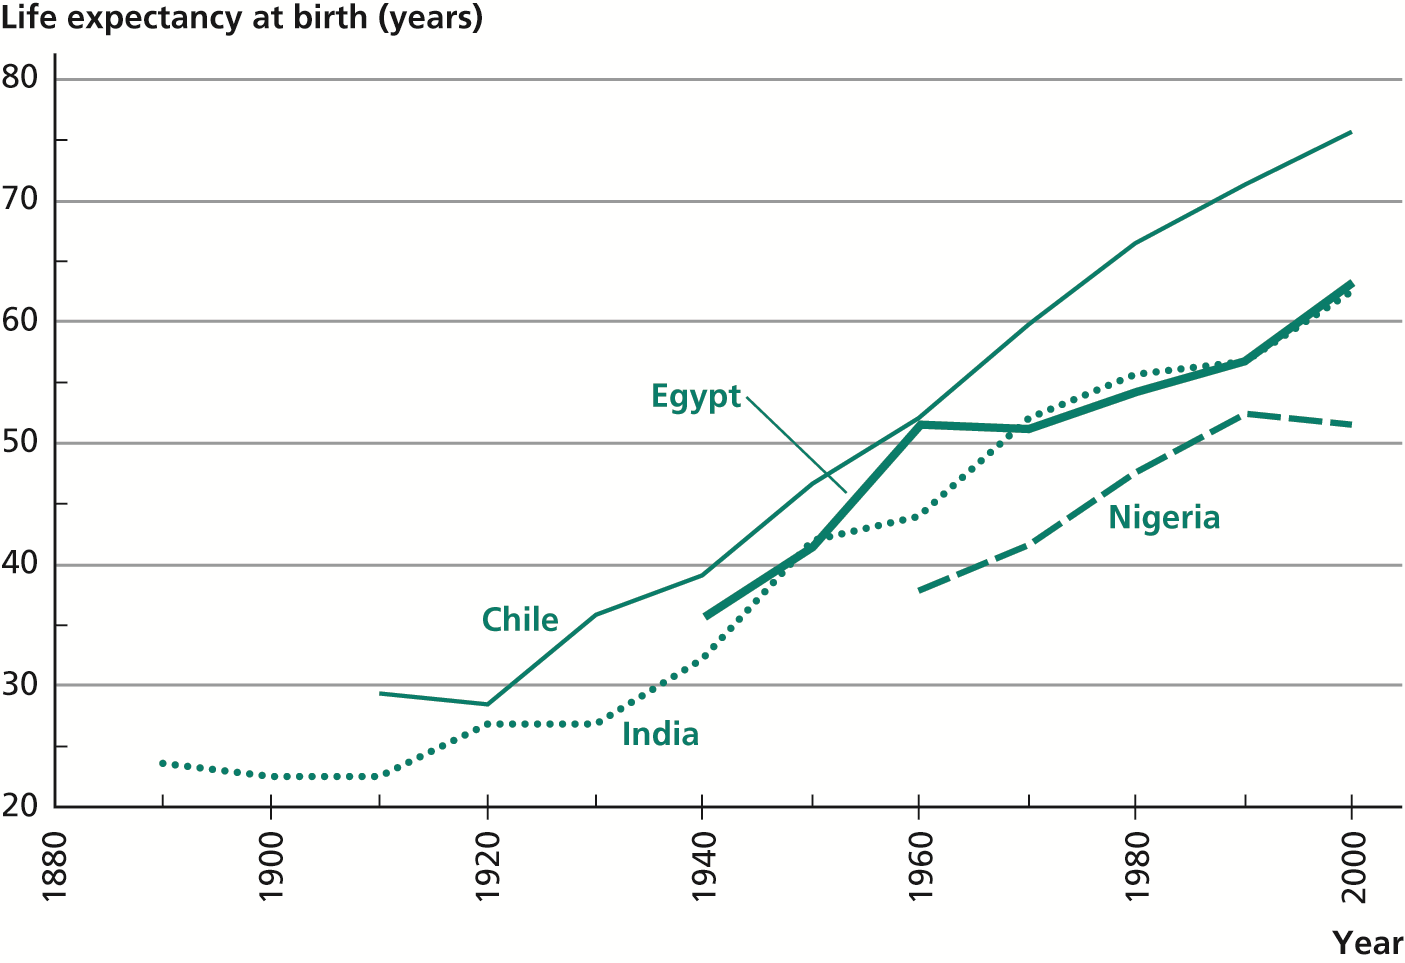
\includegraphics[width=.75\textwidth]{./img/4.9.png}
\end{center}
\end{frame}

\begin{frame}[label={sec:org6c3fe22}]{}
\alert{Fertility transition}
\begin{itemize}
\item Total fertility rate: number of children the each woman would have if she lived through child-bearing age
\item Fertility rates decreased rapidly in developed world
\item Decreasing in developing world, but still higher than developed world
\item Possible explanations:
\begin{enumerate}
\item Contraception
\item Declining mortality
\item Income and substitution effects
\item Quantity/quality tradeoff
\end{enumerate}
\end{itemize}
\end{frame}

\begin{frame}[label={sec:org0191772}]{}
\begin{center}
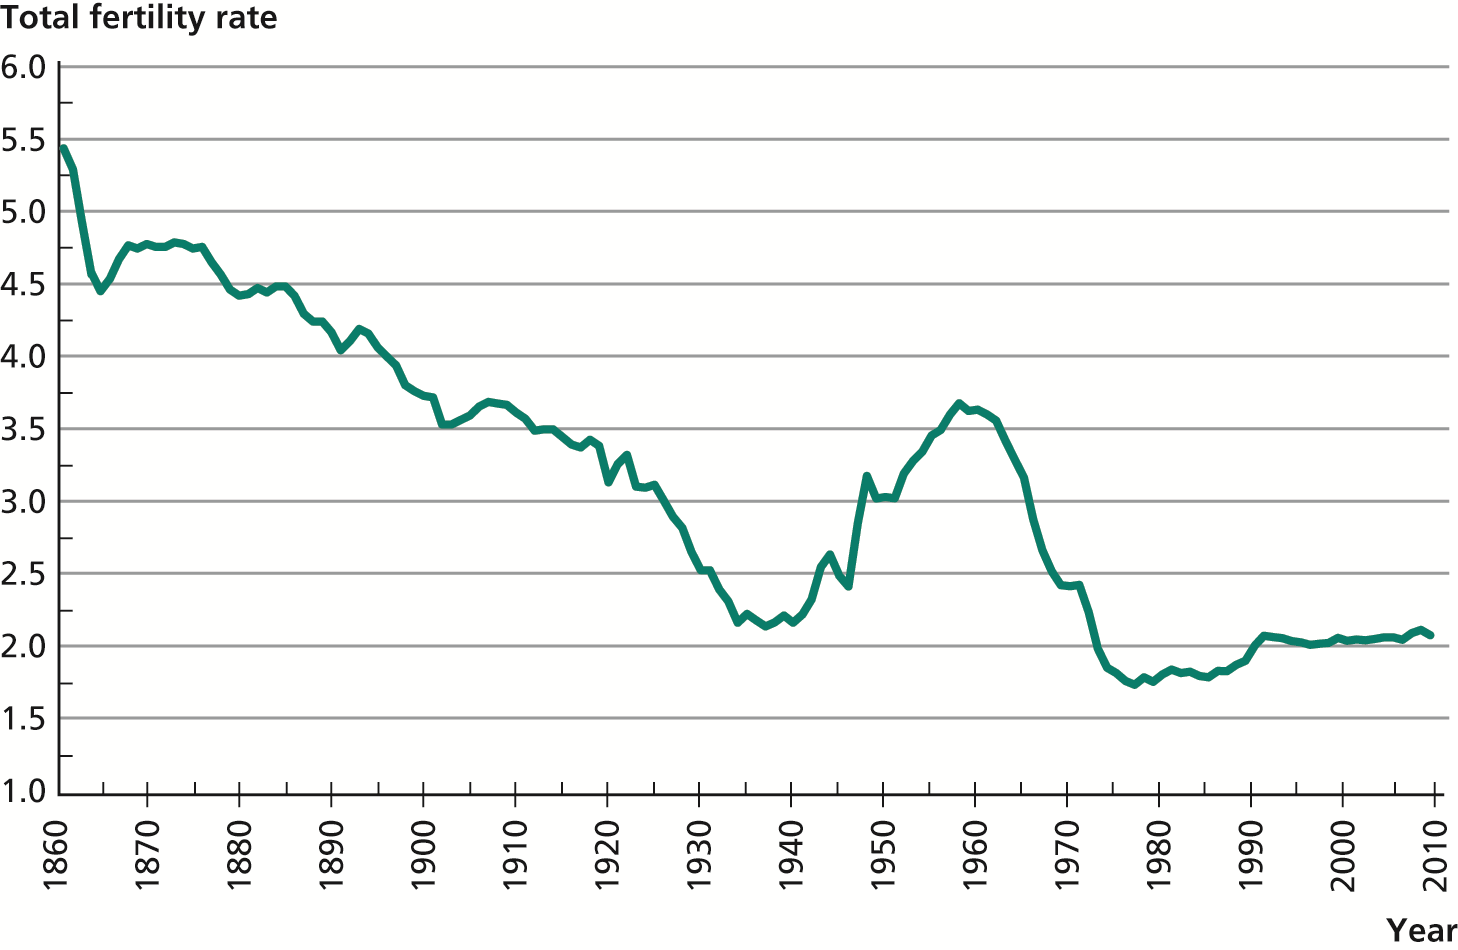
\includegraphics[width=.75\textwidth]{./img/4.10.png}
\end{center}
\end{frame}

\begin{frame}[label={sec:org53de3e1}]{}
\alert{Contraception}
\begin{itemize}
\item Fertility rates began declining in developed world long before contraception was widely available
\item Fertility in developing world decreasing contemporaneously with contraception
\item Micro studies:
\begin{itemize}
\item Making contraception available decreases number of offspring
\item Decreases unwanted pregnancies
\item Increases female "bargaining power", agency
\end{itemize}
\end{itemize}
\end{frame}

\begin{frame}[label={sec:orgeeb7e43}]{}
\alert{Mortality reduction}
\begin{itemize}
\item Perhaps parents don't care about the number of children, but rather the number that survive to adulthood
\item If mortality rates are high, parents will want more children to ensure more adult children
\item Declining mortality rates will mean fewer children, effects likely delayed
\end{itemize}
\end{frame}

\begin{frame}[label={sec:orgac12f58}]{}
\alert{Income and substitution effects}
\begin{itemize}
\item Rising income means people can afford more of everything, including children (income effect)
\item Rising income means the opportunity cost of children is higher (substitution effect)
\item If substitution effect dominates, people want fewer children as income rises
\item In developing countries, female wages generally rise faster than male, substitution effect higher for women
\end{itemize}
\end{frame}

\begin{frame}[label={sec:orgc47f778}]{}
\alert{Quantity/quality}
\begin{itemize}
\item Development increases opportunities for children
\item Parents may invest more in children's education, knowing payoffs are higher
\item This leaves less resources for other children
\item Parents choose having fewer, higher quality children
\end{itemize}
\end{frame}

\begin{frame}[label={sec:org6aa8698}]{}
\alert{Demographic transition}
\begin{itemize}
\item In general, mortality rates decline before fertility rates
\item We can model population growth as a \alert{demographic transition}
\item Falling mortality rates give rise to increasing population until fertility declines as well
\end{itemize}
\end{frame}

\begin{frame}[label={sec:org7a267de}]{}
\begin{center}
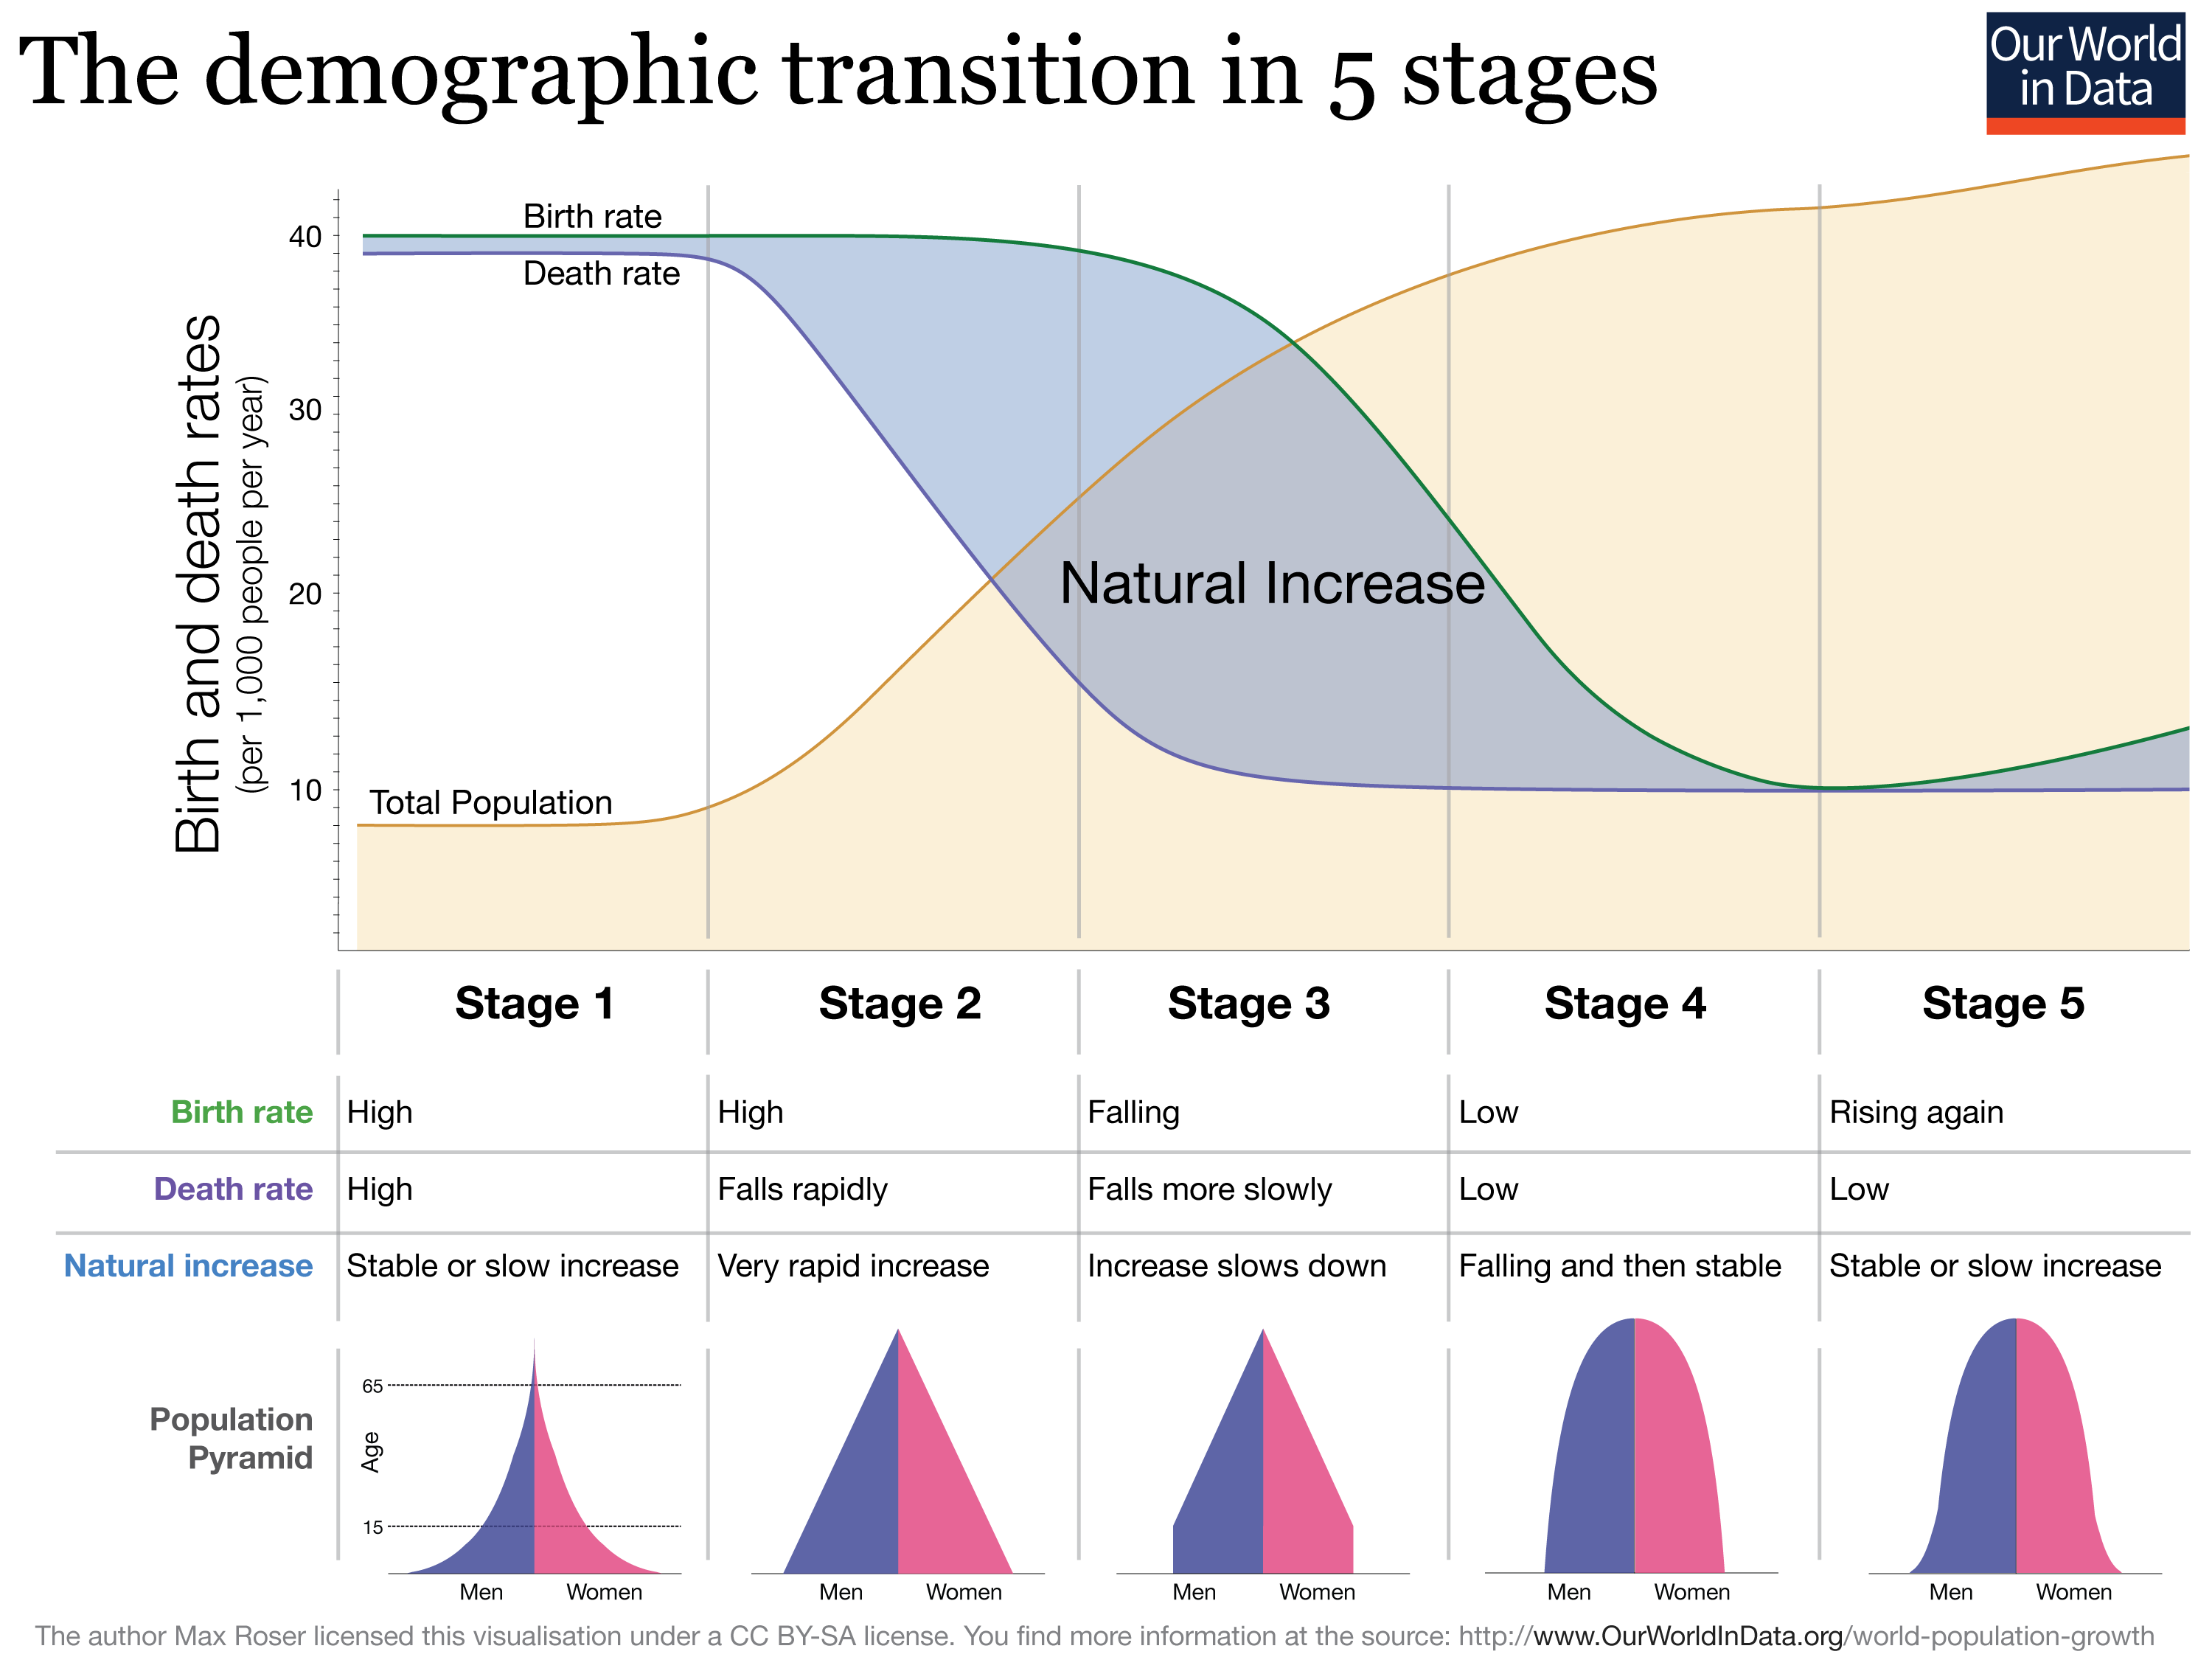
\includegraphics[width=.75\textwidth]{./img/Demographic-Transition.png}
\end{center}
\end{frame}

\begin{frame}[label={sec:org3c9ac42}]{}
\begin{center}
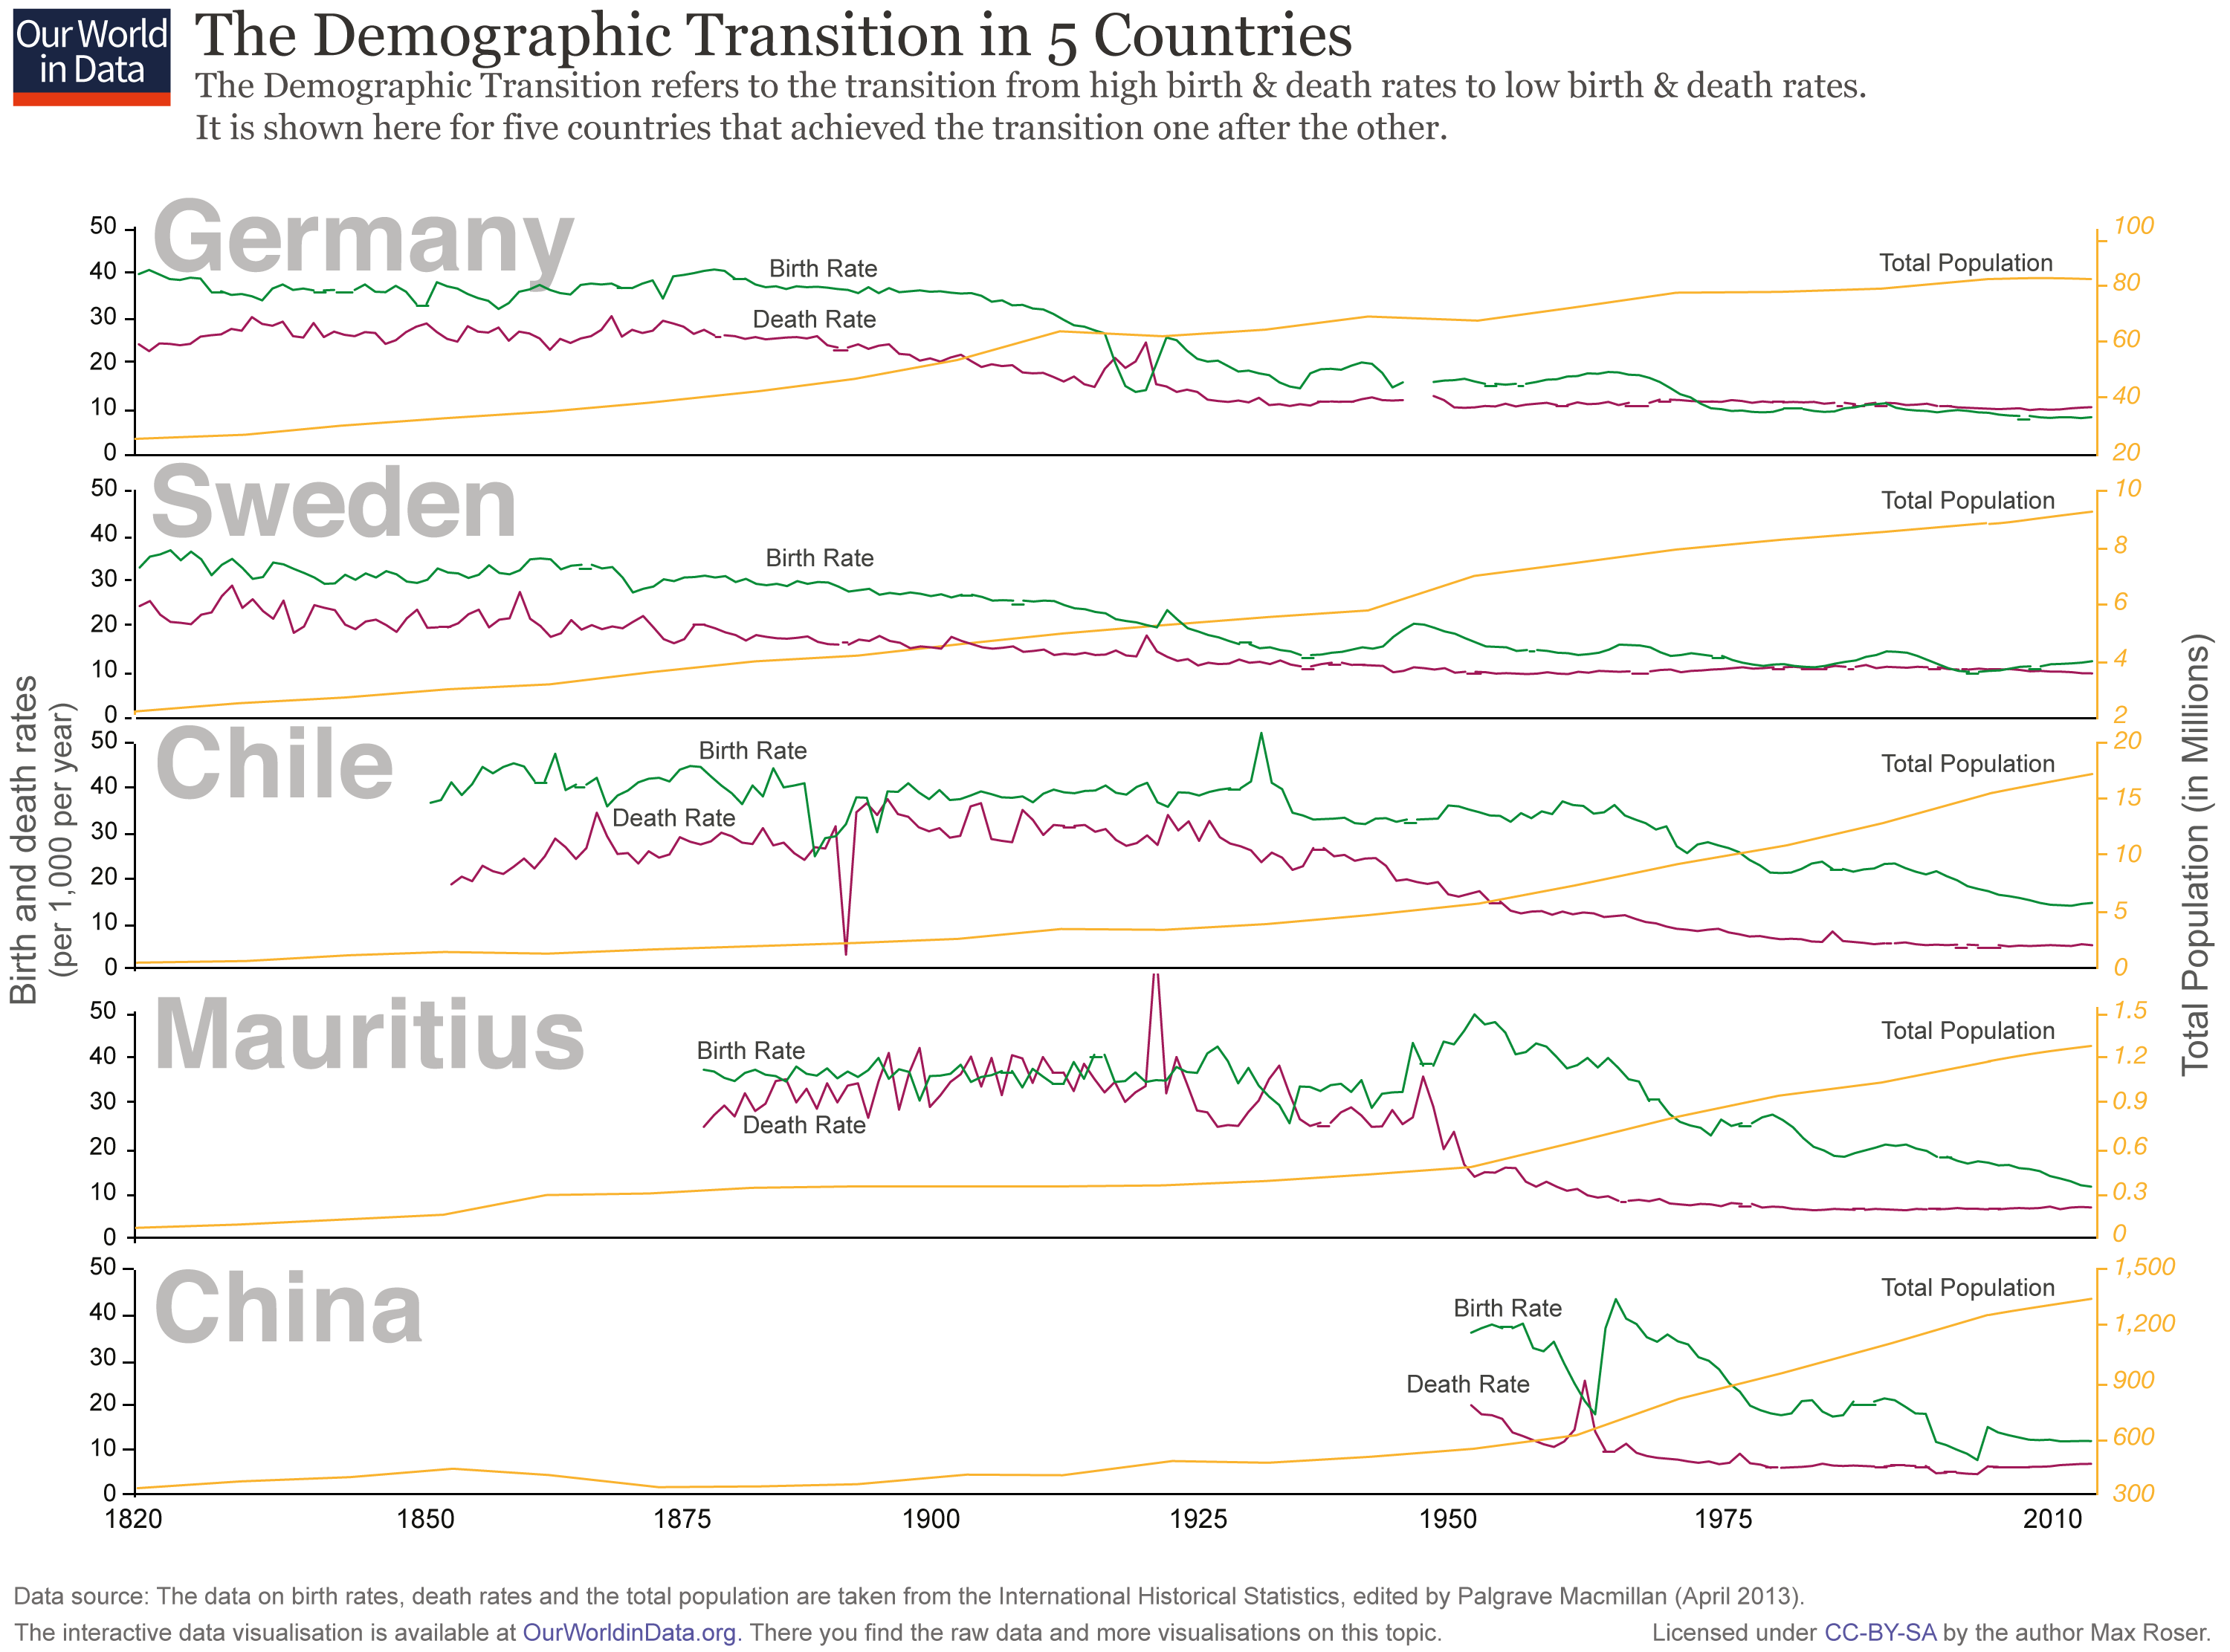
\includegraphics[width=.75\textwidth]{./img/demographic-transition-5.png}
\end{center}
\end{frame}

\begin{frame}[label={sec:org2d49e98}]{}
\url{https://ourworldindata.org/grapher/child-mortality-vs-population-growth?time=1970..2015}
\end{frame}

\begin{frame}[label={sec:org556a4bc}]{}
\alert{Fertility in the developed world}
\begin{itemize}
\item Fertility rates in many developed countries are well below "replacement level"
\item Should expect declining populations (Japan projected to lose 29\% of population by 2055)
\item Tempo effect: women delaying children can "artificially" reduce fertility rates but maintain constant population
\item Increasing wages and political freedom for women can increase tempo effects
\end{itemize}
\end{frame}

\begin{frame}[label={sec:orgf59b13f}]{}
\alert{HIV/AIDS}
\begin{itemize}
\item 90\% of infected people live in developing countries
\item 5\% of SSA infected (25\% in Botswana)
\item Reverses many of the mortality gains experienced elsewhere
\item Life expectancy \alert{decreased} 15 years in SSA
\end{itemize}
\end{frame}

\begin{frame}[label={sec:orgaa9f537}]{}
\alert{Aging}
\begin{itemize}
\item Declining mortality rates mean more people live into old age
\item Declining fertility rates mean there are fewer children
\item Median global age will increase 10 years by 2050
\item Only workers create output, retired people don't work
\end{itemize}
\end{frame}

\begin{frame}[label={sec:org3e9e334}]{}
\begin{center}
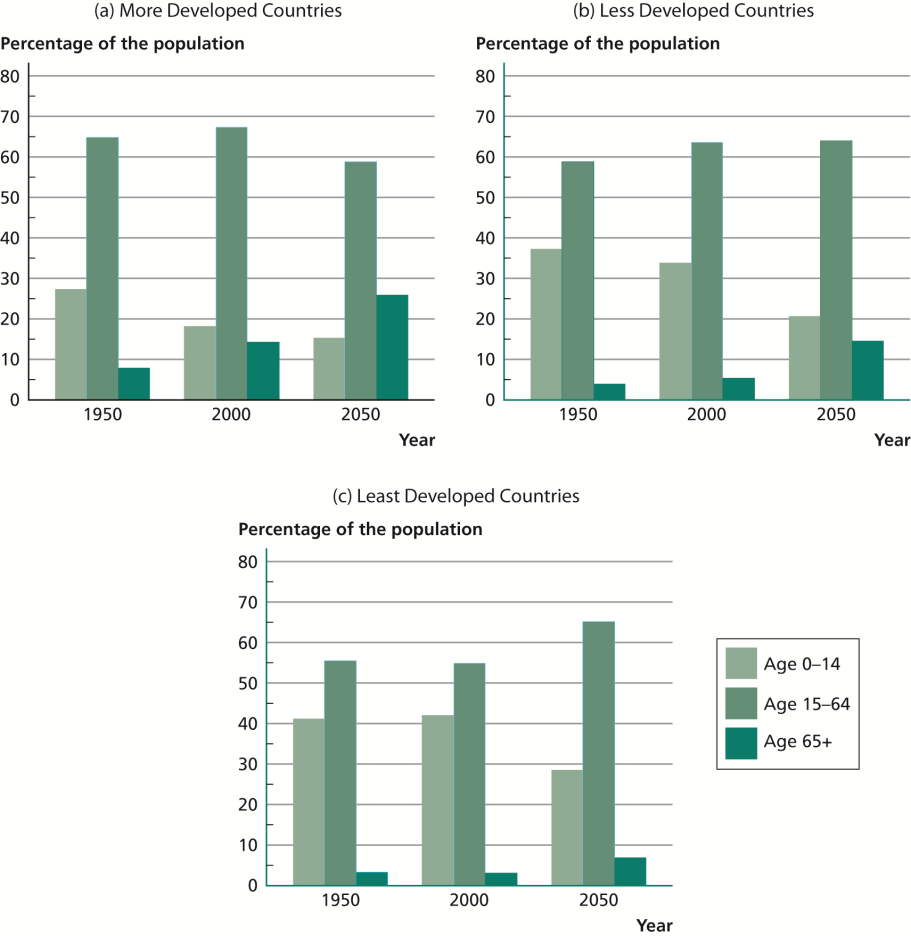
\includegraphics[width=.75\textwidth]{./img/5.6.png}
\end{center}
\end{frame}

\begin{frame}[label={sec:org4556f33}]{Working-age fraction of US population}
\begin{center}
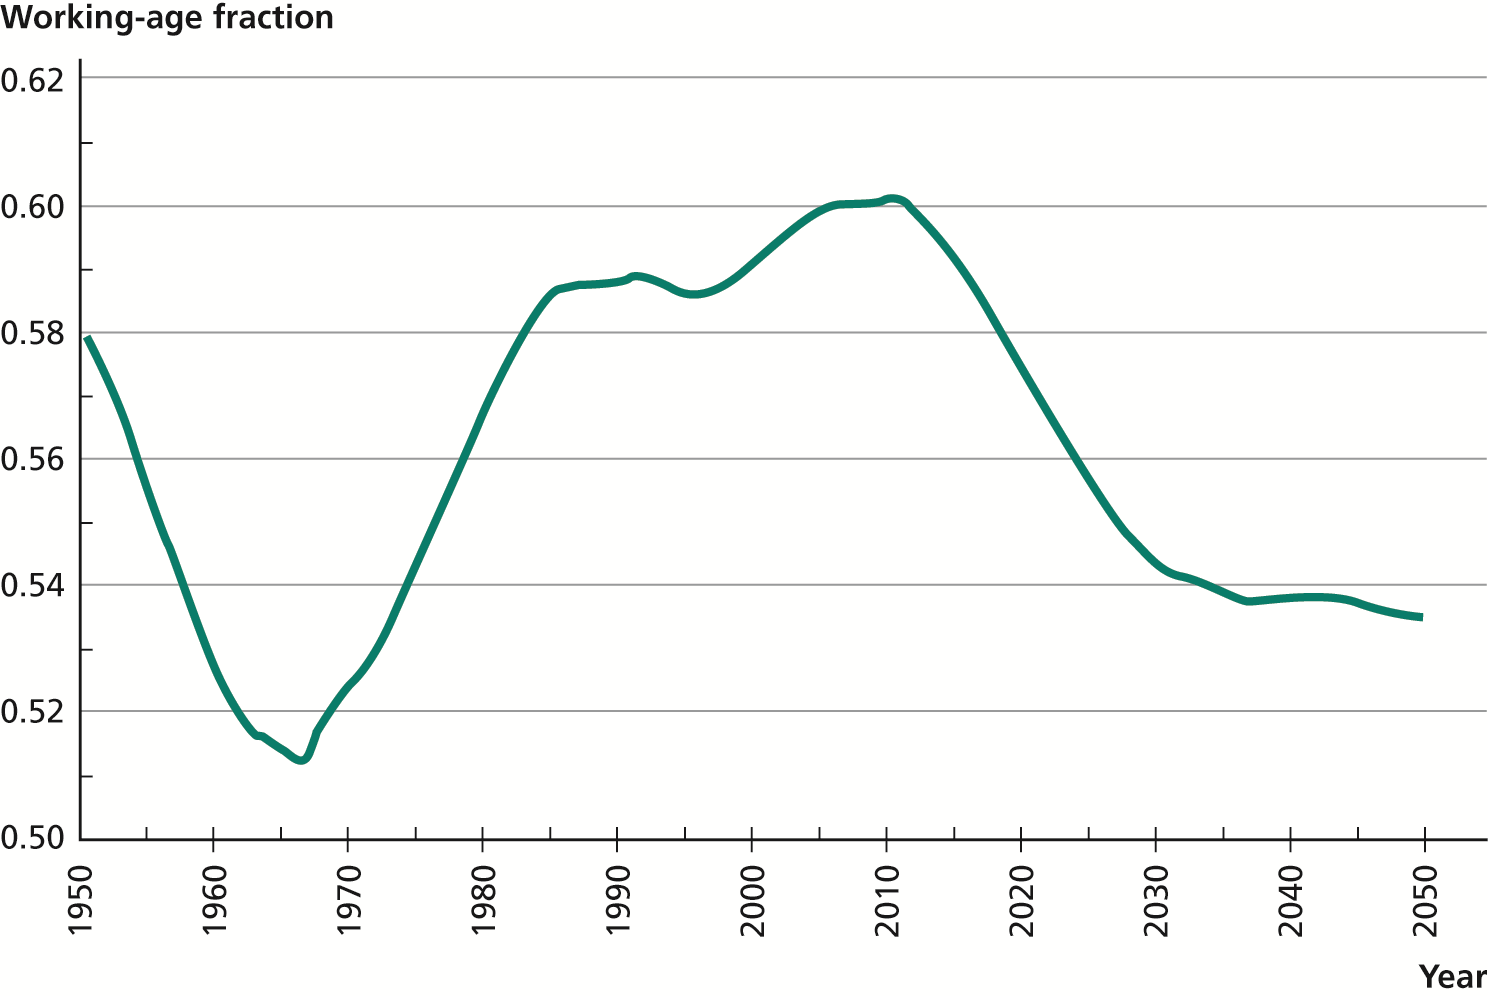
\includegraphics[width=.75\textwidth]{./img/5.7.png}
\end{center}
\end{frame}

\begin{frame}[label={sec:org9f5dec4}]{}
\alert{GDP per capita and aging}
\begin{itemize}
\item GDP per worker = GDP/(\# of workers)
\item GDP per capita = GDP/(total population)
\end{itemize}
$$\text{GDP per capita} = \dfrac{\text{GDP}}{\text{workers}} \times \dfrac{\text{workers}}{\text{population}}$$
$$\text{GDP per capita} = \text{GDP per worker} \times \dfrac{\text{workers}}{\text{population}}$$
\begin{itemize}
\item GDP per capita can decrease even as GDP per worker increases
\end{itemize}
\end{frame}
\end{document}